\section{System Features and Capabilities}

\textbf{THERAPY} is designed to be modular, extensible, and user-centric. Each component serves a specific function within the therapeutic feedback loop, contributing to emotional clarity, therapeutic continuity, and ethical data integration.

\subsection*{1. Client-Facing Features}

\begin{itemize}
  \item \textbf{Mood Check-ins} — Simple 1–10 scale entries with optional context, captured daily or on demand.
  \item \textbf{Guided Journaling} — Prompts tailored to emotional state, trauma sensitivity, or therapeutic goals.
  \item \textbf{Progress Visualizations} — Charts and trend summaries reflecting emotional fluctuations over time.
  \item \textbf{Personal Insights Feed} — Private AI-generated reflections and reframings based on journal content.
  \item \textbf{Education Portal} — Access to curated, digestible psychoeducation (CBT concepts, emotional literacy, somatic grounding).
\end{itemize}

\vspace{1em}
\begin{center}
  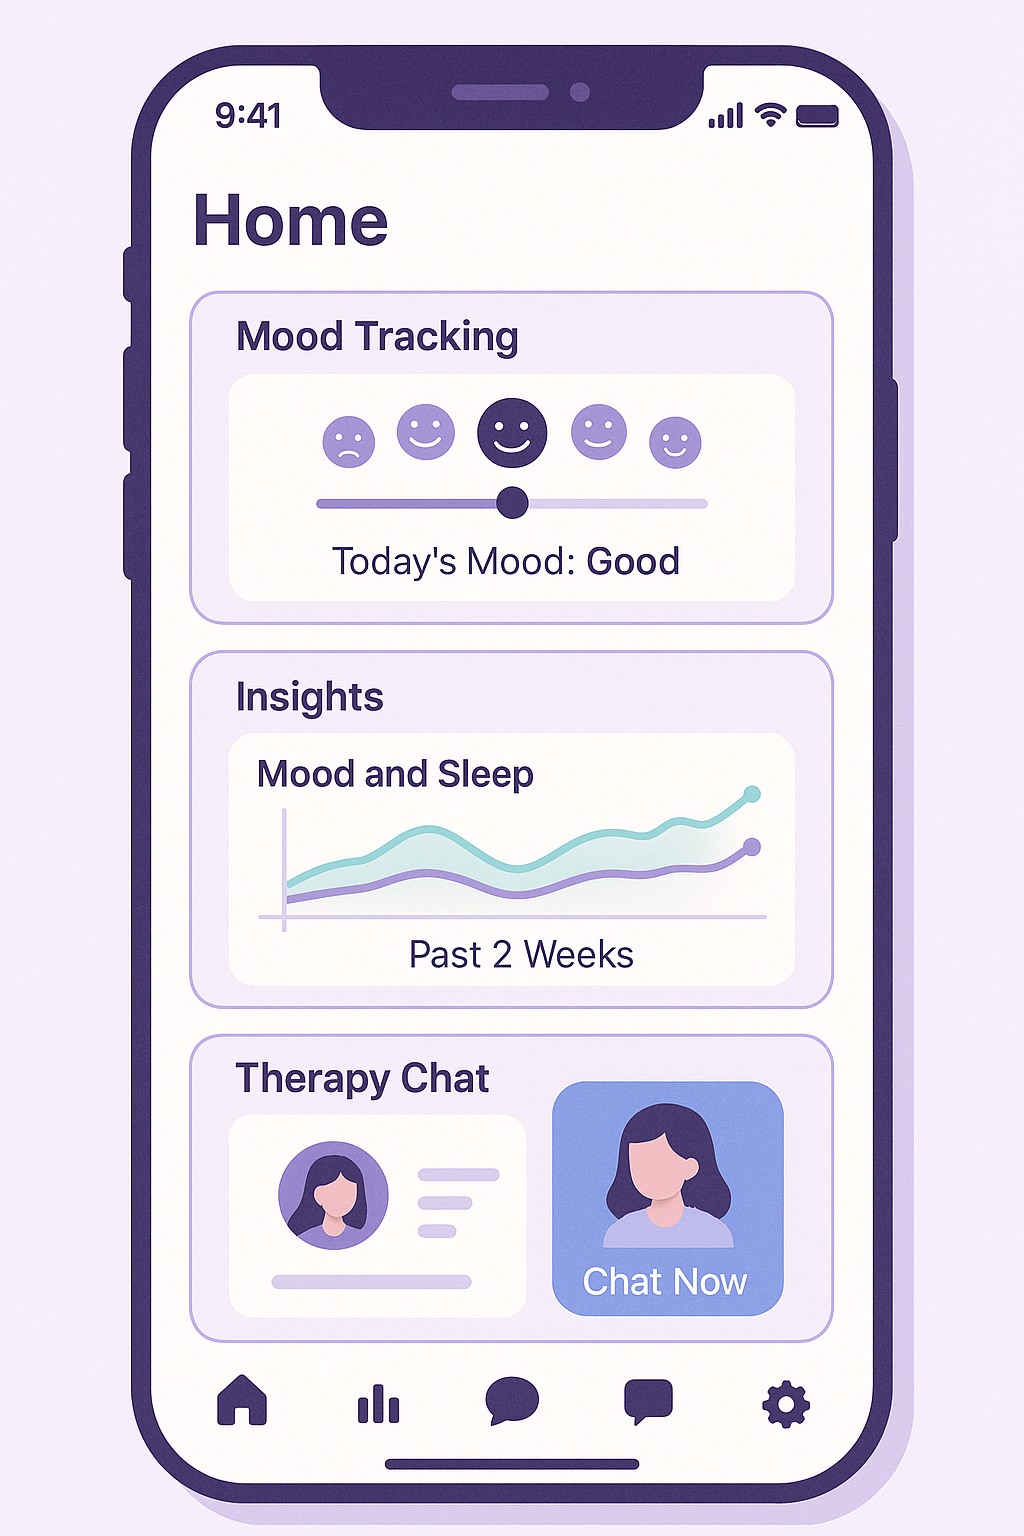
\includegraphics[width=0.85\textwidth]{features_client_mockup.png}
  \captionof{figure}{Example: Mobile interface showcasing client journaling, mood tracking, and visual feedback}
\end{center}
\vspace{2em}

\subsection*{2. Therapist Dashboard Features}

\begin{itemize}
  \item \textbf{Client Summary View} — Weekly emotional overviews, including mood trajectories, topic themes, and AI-inferred flags.
  \item \textbf{Session Preparation Feed} — Highlights key journal moments, shifts in tone, and recent cognitive distortions.
  \item \textbf{Historical Context} — Continuity timeline to revisit past patterns or unresolved therapeutic themes.
  \item \textbf{Secure Messaging (optional)} — Optional short-form messaging between sessions, scoped and rate-limited.
  \item \textbf{Insight Acknowledgement} — A private space to mark observations before or after sessions.
\end{itemize}

\vspace{1em}
\begin{center}
  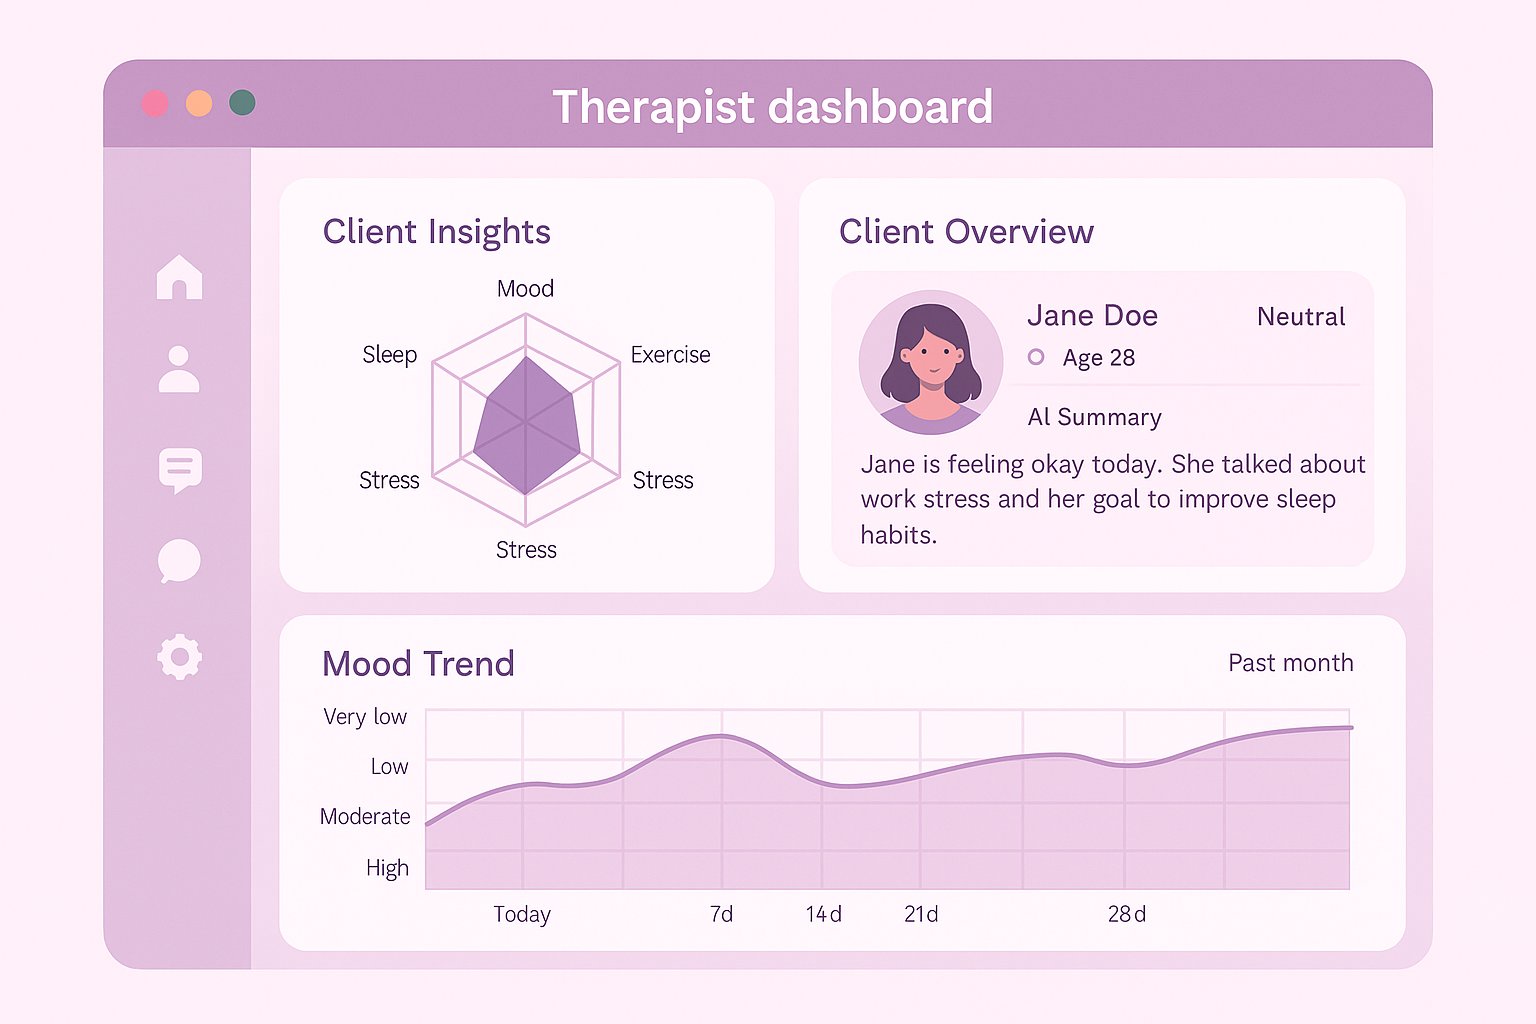
\includegraphics[width=0.85\textwidth]{features_therapist_dashboard.png}
  \captionof{figure}{Example: Therapist dashboard highlighting client emotional trends, AI flags, and journal insights}
\end{center}
\vspace{2em}

\subsection*{3. System-Level Infrastructure}

\begin{itemize}
  \item \textbf{AI Summarization Engine} — Uses large language models fine-tuned on therapeutic language and emotional tone.
  \item \textbf{Privacy-first Data Model} — End-to-end encryption, opt-in logging, and user-tuned sharing settings.
  \item \textbf{Modular API Layer} — Built for integration with third-party EHRs, clinical trial platforms, or research data lakes.
  \item \textbf{Open-Source Core} — Transparent and extensible framework for nonprofit and academic use.
\end{itemize}

\vspace{1em}
\begin{center}
  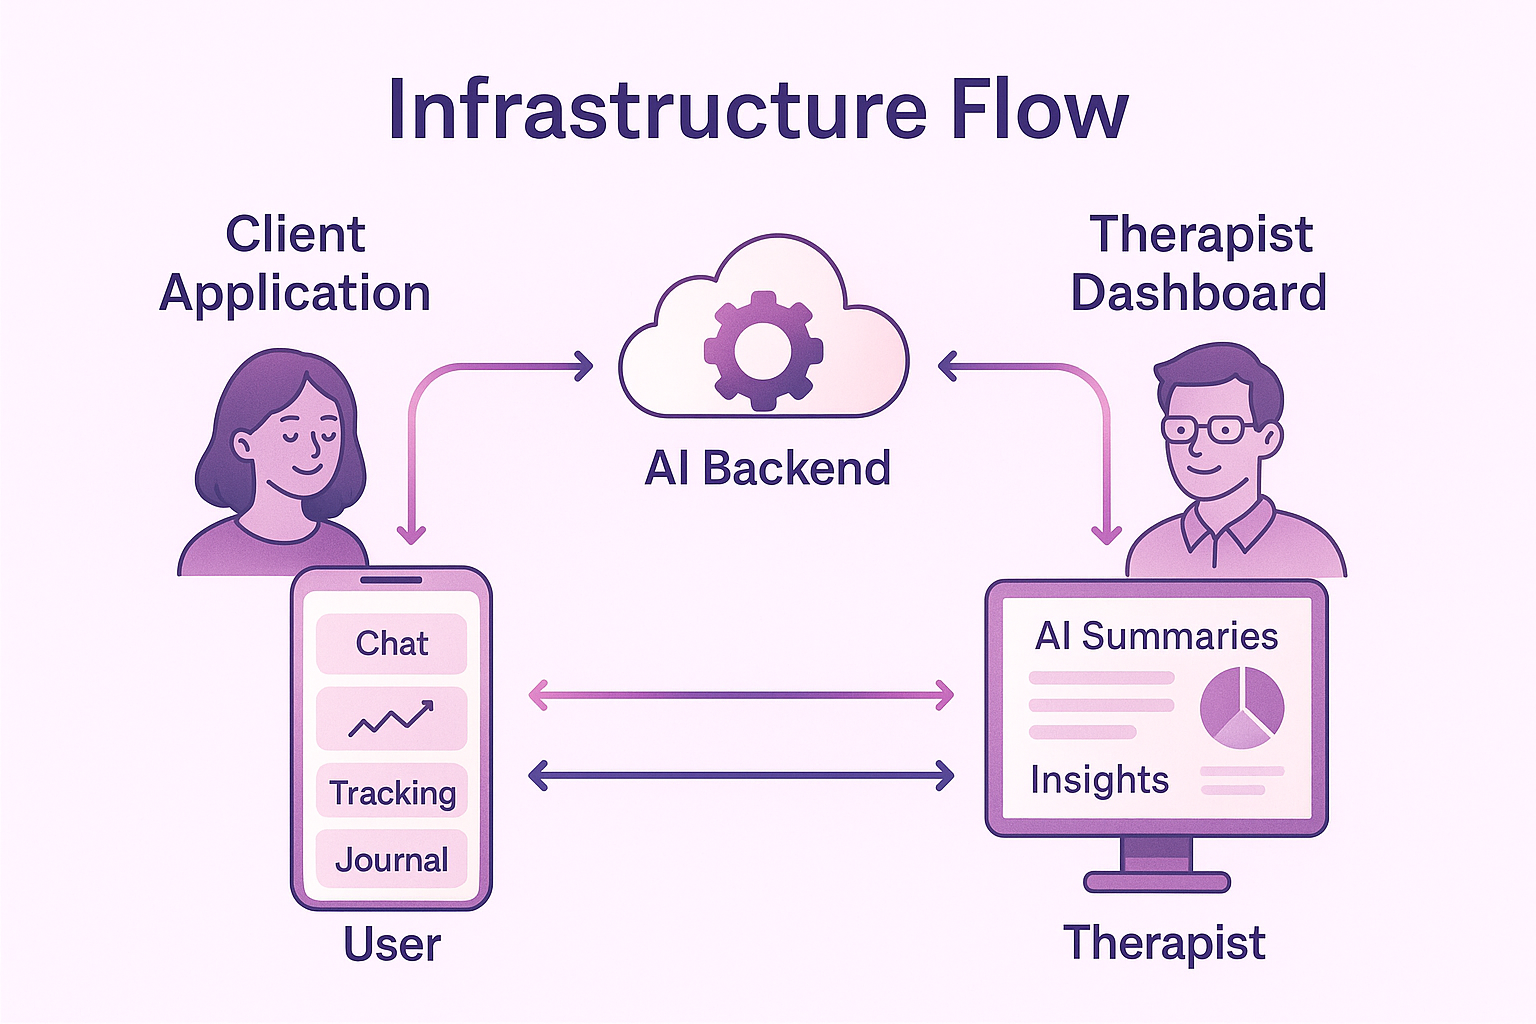
\includegraphics[width=0.85\textwidth]{features_infrastructure_flow.png}
  \captionof{figure}{Example: High-level system diagram showing THERAPY's backend architecture and data flow}
\end{center}
